\noindent \textred{1.}
{$F(x) = A (1 - e^{-bx}) u(x-a)$, where $u(x)$ is a step function. $a$ and $b$ are positive constants.
\begin{enumerate}
    \item[(1)] Find constant $A$ so that $F(x)$ is a probability distribution function. \\
    \myAnswer{
    If $F(x)$ is a probability distribution function, then we have $F(-\infty)=0$ and $F(+\infty)=1$, which yield \underline{$A=1$}.
    }
    \item[(2)] Draw $F(x)$. \\
    \myAnswer{
    To draw $F(x)$, we set $a=2, b=0.5$. \\
    }
    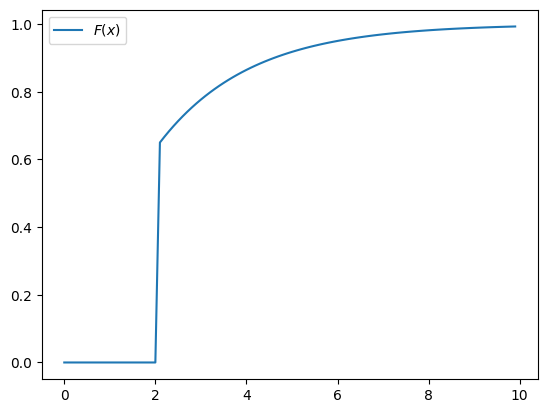
\includegraphics[width=0.5\linewidth]{HWs//HW2//figures/1-2.png}
    \item[(3)] Find and draw $f(x)$. \\
    \myAnswer{
    $f(x) = F^{'}(x) = \underline{b e^{-bx} u(x-a) + (1-e^{-ab})\delta(x-a)}$\\
    }
    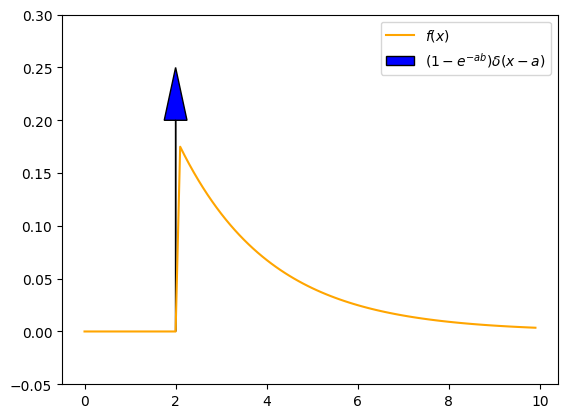
\includegraphics[width=0.5\linewidth]{HWs//HW2//figures/1-3.png}
\end{enumerate}
}
